%# -*- coding: utf-8-unix -*-
\chapter{Experiments}
\section{Dataset and Metrics}
In the field of incremental learning, there are not any publicly available datasets specialized for this problem. Following the common practices in other papers, we can artificially construct datasets for incremental learning, using publicly available machine learning datasets, by artificially hiding training data from the model and increment the data gradually. In our paper, since we focused on class-incremental learning for image classification, we follow the common practice in relevant papers to construct the incremental setting using the CIFAR-10 and CIFAR-100 image classification dataset. We can construct the dataset in the following way:
\begin{enumerate}
	\item In the beginning, assume the model can only use the first $C$ classes of data as training set. Train the model with them.
	\item Add a new class of data into the training set so that the total number of classes become $C+1$, and perform class-incremental learning algorithms. 
	\item Test the model's performance on the $C+1$ classes. Depending on the metric, we may merely consider the average accuracy for the $C+1$ classes, or require that both accuracy for the first $C$ classes and accuracy for the $C+1$-th class are high.
	\item Let $C \gets C+1$. Depending on the concrete metrics, terminate or repeat Steps 1,2,3 again until $C$ reaches the maximum number of classes in the original dataset.
\end{enumerate}



\subsection{CIFAR-10 Dataset}

The CIFAR-10 Dataset is collected by Alex and Hinton etc.\cite{krizhevsky2009learning} and maintained by the CIFAR organization. This dataset is an image classification dataset. The dataset contains sixty thousand images in total. The dataset contains 10 classes in all, and there are six thousand images belonging to each class. The images are in the size of $32 \times 32$, with RGB 3 dimensions. The dataset is divided into the training set and test set already by its creators. The training set consists of fifty thousand images, and the remaining ten thousand images belong to the test set. Each class has exactly five thousand images in the training set, and one thousand images in the test set. Since the images are very tiny, deep networks can run relatively fast on this dataset.

Typically, deep neural networks can achieve more than $90\%$ accuracy on this dataset. The state-of-the-art paper using Shake-Shake Regularization\cite{gastaldi2017shake}, achieved $2.86\%$ accuracy on this dataset. Actually they used lots of tricks and trained for a much longer time. For example, they used cyclic learning rates, and trained for four hundred epochs instead of fewer than two hundred epochs as commonly used by other papers.

\subsection{CIFAR-100 Dataset}
The CIFAR-100 Dataset is an extension to CIFAR-10 Dataset. The dataset contains sixty thousand images too. The dataset contains 100 classes in all, and there are six hundred images belonging to each class. The images are in RGB 3 dimensions. They are in the size of $32 \times 32$. The dataset is divided into the training set and test set on the website. The training set includes fifty thousand images, and the rest ten thousand images are in the test set. Each class has exactly one thousand images in the test set, and five thousand images in the training set.

Compared to CIFAR-10, this dataset has the same number of images, so the training and testing time is similar for similar networks. Since there are 100 classes, the problem becomes much harder for deep networks to recognize. Thus typically, most deep networks can only achieve about $80\%$ accuracy on this dataset. The best results up to now is also the paper \cite{gastaldi2017shake}, and they achieved $15.85\%$ accuracy.

\subsection{Evaluation Metric}

In this paper, we follow the evaluation protocol for class-incremental learning introduced in the paper ICaRL\cite{rebuffi2017icarl}. Before that paper, there does not exist any agreed benchmark protocol for evaluating class-incremental learning methods. In the protocol, we will use a multi-class image classification dataset like CIFAR-10 and CIFAR-100. Given such a dataset, the classes will be arranged in a fixed random order. To compare between each method, each method will be trained in a class-incremental way on the gradually available training data. After adding each class or adding a batch of classes at a time, the classifier will be tested on the test data part of the dataset, considering only the classes that are already been learned. Doing this, we can obtain a curve of the classification accuracies after each batch of incremented classes. We will repeat this procedure for 10 times with different random class orders and average over the curve.

\section{Experimental Setup}

In the experiments, we will evaluate our method on two representative network structures: ResNet and ShuffleNet. ResNet is the typical architecture in deep convolutional networks, while ShuffleNet is a typical network for deep learning in mobile devices with limited computation budget. By showing that these two network exhibits similar trends, we prove the robustness of our method on different kinds of deep learning network structures. 

In the following experiments, we will set the hyper-parameter $\alpha$ as 2. The hyper-parameter $\beta$ is set to 1. The learning rate, if not specified, would be 0.1 in the first half of epochs, and 0.01 in the second half of epochs. The weight decay is set to 0.0001. The momentum for the momentum-based Stochastic Gradient Descent optimizer is set to 0.9. The max epoch parameter to be used after adding each class is set to 2. Note that for $\lambda=1$ in Algorithm \ref{algo:slow}, there it will be equivalent to training for 4 epochs, because one epoch is trained in Step 1 and one epoch is trained in Step 2.

Unless specified, we present the results using Algorithm \ref{algo:slow}, because our experiment machines usually do not have such fast inference speed. A model trained from scratch will typically need 160 epochs. In the experiments, after adding one class, we only used $2~4$ epochs. Thus, our method works extremely fast, using only about $1/80$ of the computation.

\subsection{Performance on CIFAR-100 Dataset using ResNet32}

We first test the performance using ResNet. Since ICaRL used ResNet32 as their feature extractor, we use ResNet32 too, where the number 32 refers to the number of layers. We follow the concrete dimensions and structure used in the ResNet paper\cite{he2016deep}. We first present the results on CIFAR-100 Dataset, because the relevant paper, ICaRL, did not test their results on CIFAR-10. We incremented one class at a time. But ICaRL worked poorly when incrementing one class at a time perhaps due to the preferences of their algorithm, so we used their results when every time a batch of 10 new class of data arrives. 

\begin{figure}[!htp]
	\centering
	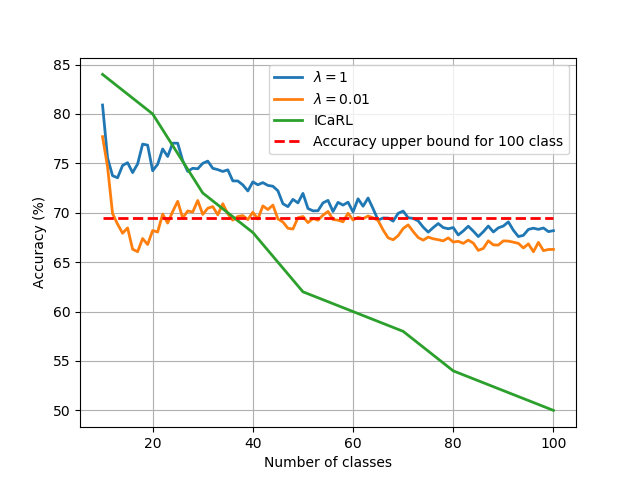
\includegraphics[width=12cm]{cifar100.png}
	\bicaption[Performance comparison on CIFAR-100 Dataset]
	{CIFAR-100数据集上表现对比}
	{Performance comparison on CIFAR-100 Dataset}
	\label{fig:cifar100}从
\end{figure}


As shown in Fig.~\ref{fig:cifar100}, our algorithm outperform ICaRL by a large margin. Our parameter $\lambda$, controls the number of hard examples chosen to train the model in Step 2. In the most extreme case $\lambda = 1$, the accuracy of our algorithm becomes very close to the performance upper bound when all 100 classes of data are used to train the deep neural network from scratch. By using $\lambda=0.01$, we are using approximately $1/2$ computation compared to $\lambda=1$, because by comparing the amount data used by Step 1 and Step 2 in total, we can write the comparison by the ratio $\frac{1+1}{1+0.01} \approx 2$. The smaller amount of computation leads to slightly worse performance. As revealed, with higher $\lambda$, we can obtain higher accuracy, but spending more computation time. With lower $\lambda$, we save more computation time, by will degrade some accuracy.

In the beginning when there are fewer than 30 classes, the accuracy of ICaRL algorithm is higher than us. We suspect that they might have used a larger network than us, so they can have higher accuracy before incremental learning happens when there are initially 10 classes. Another reason might be their classification algorithm does better when the class number is low, because they used a quite complicated classification algorithm. This problem does not matter too much, because the most important aspect in incremental learning is the trend of the curve, and not the initial accuracy.

There is also an interesting trend shown in our curves. During the 10 to 25 classes, the accuracy of our algorithm first drops a little, and then goes up. The reason why the accuracy first drops is that it is easier for the neural network to correctly classify fewer classes. But at the same time, more classes provide stronger regularization power, so the network can learn more general features and does not overfit. Therefore, the accuracy goes up a little. This phenomenon is similar to the discoveries in multi-task learning, joint training, etc. 

Average values might not truly reflect the knowledge the model has learned. Next, we want to see whether the accuracies of each class are high enough, so that the network really learned knowledge for every class, instead of biasing towards specific classes. Shown in Table \ref{tab:cifar100}, we do not see obvious bias for specific classes using our algorithm. This indicates that our algorithm is able to learn knowledge for every class effectively. Note that the accuracy varies quite a lot for different classes, from $45\%$ to $85\%$. This is because the difficulty of recognizing every class is different.
\begin{table}[!hpb]
	\centering
	\bicaption[The per-class accuracy in CIFAR-100 results]
	{CIFAR-100结果中各类别准确率}
	{The per-class accuracy in CIFAR-100 results}
	\label{tab:firstone}
	\begin{tabular}{@{}lp{10cm}@{}} \toprule
		Case &  Final accuracy on each of the 100 classes ($\%$)\\ \midrule
		Model trained from scratch  &[83.0, 82.0, 51.0, 48.0, 52.0, 73.0, 77.0, 72.0, 80.0, 79.0, 57.0, 46.0, 78.0, 62.0, 63.0, 75.0, 73.0, 78.0, 62.0, 61.0, 80.0, 86.0, 63.0, 78.0, 79.0, 58.0, 73.0, 59.0, 76.0, 71.0, 65.0, 61.0, 61.0, 66.0,
		75.0, 52.0, 75.0, 79.0, 54.0, 81.0, 64.0, 82.0, 75.0, 72.0, 49.0, 59.0, 49.0, 61.0, 93.0, 84.0, 51.0, 70.0, 64.0, 86.0, 77.0, 41.0, 83.0, 78.0, 83.0, 66.0, 83.0, 66.0, 73.0, 70.0, 51.0, 53.0, 76.0, 58.0,
		87.0, 73.0, 63.0, 76.0, 46.0, 60.0, 57.0, 80.0, 86.0, 62.0, 64.0, 68.0, 51.0, 76.0, 86.0, 60.0, 66.0, 77.0, 69.0, 83.0, 74.0, 81.0, 79.0, 75.0, 58.0, 53.0, 91.0, 66.0, 68.0, 74.0, 47.0, 64.0]\\
		$\lambda=1$  &[82.0, 77.0, 62.0, 45.0, 53.0, 73.0, 75.0, 60.0, 86.0, 80.0, 52.0, 43.0, 74.0, 59.0, 69.0, 66.0, 76.0, 82.0, 57.0, 64.0, 81.0, 80.0, 66.0, 83.0, 81.0, 59.0, 65.0, 67.0, 80.0, 68.0, 66.0, 57.0, 67.0, 66.0, 72.0, 53.0, 79.0, 67.0, 60.0, 88.0, 60.0, 82.0, 71.0, 76.0, 46.0, 53.0, 50.0, 52.0, 92.0, 84.0, 49.0, 75.0, 69.0, 88.0, 83.0, 53.0, 81.0, 80.0, 79.0, 66.0, 86.0, 68.0, 72.0, 55.0, 54.0, 57.0, 67.0, 60.0, 88.0, 76.0, 63.0, 79.0, 42.0, 49.0, 50.0, 85.0, 88.0, 62.0, 53.0, 71.0, 43.0, 74.0, 85.0, 51.0, 68.0, 81.0, 74.0, 76.0, 75.0, 81.0, 81.0, 70.0, 54.0, 59.0, 84.0, 70.0, 55.0, 68.0, 48.0, 68.0]
		\\
		$\lambda=0.01$  & [85.0, 82.0, 59.0, 45.0, 57.0, 69.0, 73.0, 71.0, 80.0, 85.0, 53.0, 48.0, 77.0, 64.0, 56.0, 67.0, 72.0, 85.0, 63.0, 61.0, 81.0, 85.0, 65.0, 71.0, 82.0, 58.0, 62.0, 54.0, 79.0, 65.0, 53.0, 72.0, 71.0, 62.0, 72.0, 45.0, 76.0, 71.0, 60.0, 84.0, 61.0, 80.0, 68.0, 68.0, 40.0, 46.0, 35.0, 49.0, 93.0, 77.0, 49.0, 65.0, 65.0, 87.0, 83.0, 47.0, 83.0, 73.0, 75.0, 66.0, 85.0, 67.0, 61.0, 59.0, 34.0, 53.0, 74.0, 51.0, 85.0, 79.0, 59.0, 75.0, 41.0, 37.0, 50.0, 81.0, 83.0, 57.0, 54.0, 64.0, 45.0, 74.0, 84.0, 62.0, 67.0, 78.0, 68.0, 78.0, 76.0, 80.0, 74.0, 79.0, 45.0, 49.0, 89.0, 63.0, 63.0, 59.0, 48.0, 70.0]\\ \bottomrule
\label{tab:cifar100}
	\end{tabular}
\end{table}

\subsection{Performance on CIFAR-100 Dataset using MobileNetV2}

To show the effectiveness of our algorithm on other deep learning network structures, we selected another network, MobileNetV2\cite{sandler2018inverted}, to evaluate our algorithm. MobileNetV2 is a state-of-the-art network structure for mobile devices, designed to be small and efficient.

In the MobileNetV2 paper, they only ran experiments on ImageNet, and they did not design any concrete model for CIFAR datasets. Thus, we followed their practice and designed the structure ourselves, to let the network be suitable for CIFAR dataset. Our MobileNetV2 structure is shown in Table \ref{tab:mobilenetv2}. We used the same notations as their paper. $t$ refers to the expansion factor applied to the input size. $c$ refers to the output channels of every layer in the same stage. $n$ refers to how many time the basic MobileNetV2 block is repeated in the stage. $s$ refers to the total stride of the stage. $k$ refers to the number of output classes. In CIFAR-10, $k=10$, and in CIFAR-100, $k=100$.
\begin{table}[!hpb]
	\centering
	\bicaption[Our MobileNetV2 model architecture for CIFAR]
	{用在CIFAR数据集上的MobileNetV2结构}
	{Our MobileNetV2 model architecture for CIFAR}
	\label{tab:mobilenetv2}
	\begin{tabular}{@{}llllll@{}} \toprule
		Input & Operator & $t$ & $c$ & $n$ & $s$\\ \midrule
		$32^2\times3$ & conv2d & - &32&1&2\\ 
		$16^2\times32$ & bottleneck & 1 &16&1&1\\ 
		$16^2\times16$ & bottleneck & 6 &24&2&1\\ 
		$16^2\times24$ & bottleneck & 6 &32&3&2\\ 
		$8^2\times32$ & bottleneck & 6 &64&4&2\\ 		
		$4^2\times64$ & bottleneck & 6 &96&3&1\\ 
		$4^2\times96$ & avgpool $4\times4$ & - &-&1&-\\ 	
		$1\times1\times k$ & fully-connected layer & - &$k$&-&-\\ 				
		\bottomrule
		\label{tab:cifar100_mobile}
	\end{tabular}
\end{table}
\begin{figure}[!htp]
	\centering
	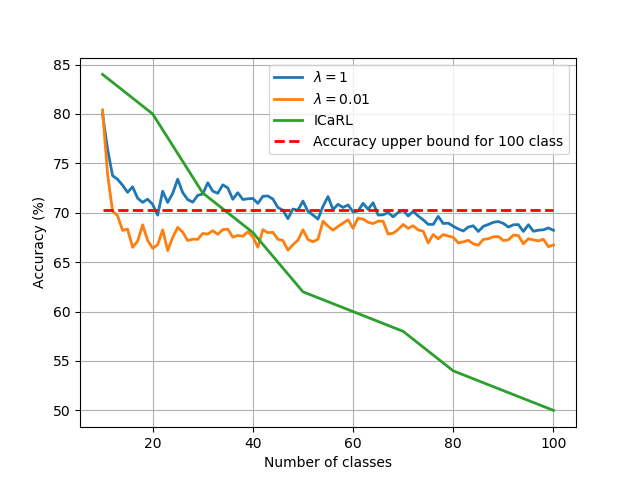
\includegraphics[width=12cm]{cifar100_mobile.png}
	\bicaption[Performance comparison on CIFAR-100 Dataset with MobileNetV2]
	{用MobileNetV2网络在CIFAR-100数据集上表现}
	{Performance comparison on CIFAR-100 Dataset with MobileNetV2}
	\label{fig:cifar100_mobile}
\end{figure}


Fig.~\ref{fig:cifar100_mobile} shows the accuracy of the model as more and more classes are added one by one. As we can see, the curves exhibit similar behaviour compared to ResNet32. We did not compare with ICaRL because they only tested on ResNet. Same with ResNet, with lower $\lambda$, we will degrade some accuracy, but we save more computation time. With higher $\lambda$, we spend more computation time, but we can obtain higher accuracy. The highest accuracy when $\lambda=1$ gives near to optimal accuracy.

Next, we also show the accuracies of each class after all 100 classes are added. Shown in Table \ref{tab:cifar100_mobile}, we see that our algorithm can let the model learn to recognize each class. The model do not have bias towards specific classes.
\begin{table}[!hpb]
	\centering
	\bicaption[The per-class accuracy in CIFAR-100 results with MobileNetV2]
	{CIFAR-100结果中各类别准确率}
	{The per-class accuracy in CIFAR-100 results with MobileNetV2}
	\label{tab:firstone}
	\begin{tabular}{@{}lp{10cm}@{}} \toprule
		Case &  Final accuracy on each of the 100 classes ($\%$)\\ \midrule
		$\lambda=1$  &[90.0, 83.0, 57.0, 40.0, 59.0, 71.0, 79.0, 67.0, 86.0, 73.0, 49.0, 49.0, 83.0, 61.0, 60.0, 68.0, 67.0, 89.0, 67.0, 53.0, 85.0, 84.0, 60.0, 79.0, 83.0, 63.0, 69.0, 64.0, 77.0, 66.0, 58.0, 70.0, 65.0, 63.0, 75.0, 32.0, 69.0, 72.0, 55.0, 85.0, 61.0, 85.0, 71.0, 77.0, 44.0, 55.0, 47.0, 55.0, 94.0, 81.0, 54.0, 72.0, 72.0, 88.0, 83.0, 49.0, 78.0, 75.0, 76.0, 71.0, 85.0, 71.0, 73.0, 62.0, 55.0, 58.0, 68.0, 58.0, 93.0, 78.0, 67.0, 79.0, 40.0, 50.0, 55.0, 83.0, 92.0, 62.0, 56.0, 75.0, 48.0, 74.0, 89.0, 63.0, 66.0, 75.0, 67.0, 72.0, 73.0, 82.0, 75.0, 72.0, 61.0, 49.0, 88.0, 67.0, 61.0, 62.0, 38.0, 67.0]
		
		\\
		$\lambda=0.01$  & [87.0, 84.0, 58.0, 38.0, 54.0, 71.0, 80.0, 71.0, 80.0, 78.0, 44.0, 43.0, 80.0, 54.0, 56.0, 69.0, 69.0, 81.0, 67.0, 62.0, 82.0, 82.0, 65.0, 80.0, 80.0, 55.0, 60.0, 51.0, 80.0, 62.0, 65.0, 72.0, 65.0, 58.0, 67.0, 50.0, 75.0, 63.0, 57.0, 82.0, 58.0, 86.0, 75.0, 79.0, 40.0, 53.0, 46.0, 58.0, 88.0, 79.0, 46.0, 71.0, 64.0, 87.0, 80.0, 44.0, 84.0, 74.0, 77.0, 52.0, 87.0, 67.0, 70.0, 56.0, 52.0, 48.0, 73.0, 53.0, 88.0, 72.0, 76.0, 83.0, 45.0, 41.0, 43.0, 86.0, 87.0, 56.0, 61.0, 73.0, 44.0, 75.0, 86.0, 53.0, 65.0, 77.0, 69.0, 81.0, 67.0, 83.0, 75.0, 72.0, 60.0, 48.0, 88.0, 62.0, 67.0, 64.0, 39.0, 64.0]
		
		\\ \bottomrule
		\label{tab:cifar100_mobile}
	\end{tabular}
\end{table}
\subsection{Performance on CIFAR-10 Dataset}
We also tested our method on the CIFAR-10 Dataset. The setting is the same, i.e., we set max epoch to be 4 when we add every class. The curves are shown in Fig~\ref{fig:cifar10-resnet} and Fig.~\ref{fig:cifar10-mobilenetv2}.



We can see that the curves are very similar to the curves compared to CIFAR-100. This shows the robustness of our method under different datasets. It is worth noting that this time our model performs further worse than the accuracy upper bound. This is due to lack of training time, since training 10 class from scratch takes 160 epochs, while we only used at most $10 \times 4 = 40$ epochs. We believe our curve would be higher when we increased the training time.
\begin{figure}[!htp]
	\centering
	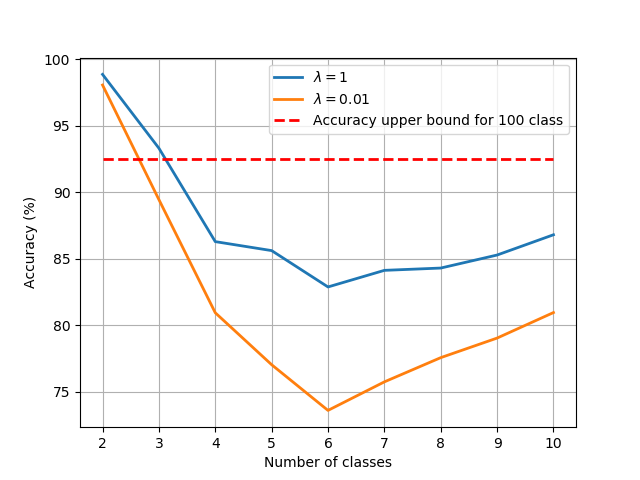
\includegraphics[width=12cm]{cifar10-resnet.png}
	\bicaption[Evaluation result on CIFAR-10 Dataset with ResNet32]
	{用ResNet32网络在CIFAR-10数据集上表现}
	{Evaluation result on CIFAR-10 Dataset with ResNet32}
	\label{fig:cifar10-resnet}
\end{figure}
\begin{figure}[!htp]
	\centering
	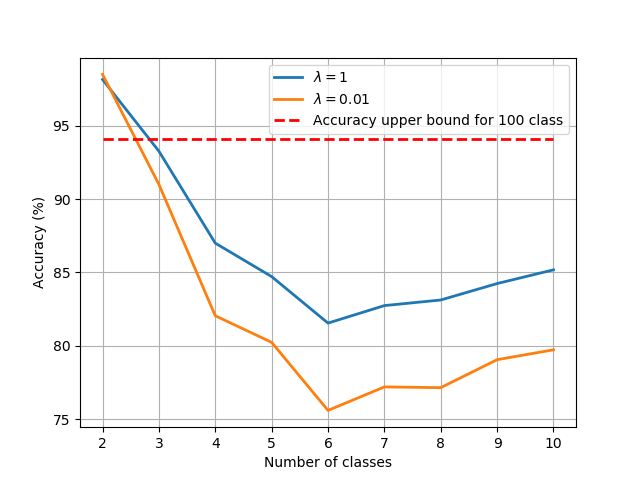
\includegraphics[width=12cm]{cifar10-mobilenetv2.png}
	\bicaption[Evaluation result on CIFAR-10 Dataset with MobileNetV2]
	{用MobileNetV2网络在CIFAR-10数据集上表现}
	{Evaluation result on CIFAR-10 Dataset with MobileNetV2}
	\label{fig:cifar10-mobilenetv2}
\end{figure}
We also show tested the per-class accuracy in Table \ref{cifar10_resnet} and Table \ref{cifar10_mobilenetv2}, to see that our model learns knowledge for every class.
\begin{table}[!hpb]
	\centering
	\bicaption[The per-class accuracy in CIFAR-10 results for ResNet20]
	{ResNet20在CIFAR-10结果中各类别准确率}
	{The per-class accuracy in CIFAR-10 results for ResNet20}
	\label{tab:firstone}
	\begin{tabular}{@{}lp{10cm}@{}} \toprule
		Case &  Final accuracy on each of the 100 classes ($\%$)\\ \midrule
		$\lambda=1$  &[88.5, 94.1, 82.3, 65.8, 87.3, 84.9, 89.0, 89.9, 93.4, 92.7]
		\\
		$\lambda=0.01$  & [85.5, 91.4, 70.7, 63.8, 79.8, 76.0, 85.4, 80.8, 89.0, 87.0]\\ \bottomrule
		\label{tab:cifar10_resnet}
	\end{tabular}
\end{table}

\begin{table}[!hpb]
	\centering
	\bicaption[The per-class accuracy in CIFAR-10 results for MobileNetV2]
	{MobileNetV2在CIFAR-10结果中各类别准确率}
	{The per-class accuracy in CIFAR-10 results for MobileNetV2}
	\label{tab:firstone}
	\begin{tabular}{@{}lp{10cm}@{}} \toprule
		Case &  Final accuracy on each of the 100 classes ($\%$)\\ \midrule
		$\lambda=1$  &[88.1, 93.3, 79.8, 68.7, 86.9, 77.4, 88.8, 88.4, 91.7, 88.7]
		
		\\
		$\lambda=0.01$  & [83.3, 91.9, 72.6, 64.7, 79.4, 67.9, 87.0, 80.4, 86.0, 84.1]
		\\ \bottomrule
		\label{tab:cifar10_mobilenetv2}
	\end{tabular}
\end{table}
\subsection{Under negligible inference speed}
We also tested our Algorithm \ref{algo:fast} under negligible inference speed. We used ResNet32 to evaluate. Since time and computational resource is limited, we are unable plot the whole curve. As an alternative, we first train the model using the first 99 classes from scratch. Then, we add the 100-th class and perform our incremental learning algorithm. We will compare the average accuracy for 100 classes, as well as per-class accuracy to evaluate our algorithm.

We compared our algorithm with the baseline algorithm Algorithm \ref{algo:baseline}. For all tests, we used a constant learning rate of $0.01$. The max epoch parameter is set to 4. However, we should note that, since the time of Step 1 can be neglected, the time consumption is much more smaller. Compared to training on the full epoch, our speed up ratio can be calculated as
\begin{align}
\eta = \frac{99+1}{\lambda \times 99 + 1} \approx \frac{1}{\lambda}
\end{align}
Thus, the speed up is almost proportional to $1/\lambda$. In the following, we tested the results for $\lambda=0.1$ and $\lambda=0.01$.

\begin{table}[!hpb]
	\centering
	\bicaption[The results]
	{CIFAR-100结果中各类别准确率}
	{The per-class accuracy in CIFAR-100 results with MobileNetV2}
	\label{tab:firstone}
	\begin{tabular}{@{}lllp{8cm}@{}} \toprule
		Algorithm & $\lambda$ &Avg. Accuracy&  Final accuracy on each of the 100 classes ($\%$)\\ \midrule
		Baseline&$\lambda=0.01$&  44.58& [72.0, 55.0, 42.0, 26.0, 23.0, 58.0, 47.0, 54.0, 41.0, 66.0, 8.0, 39.0, 45.0, 48.0, 19.0, 48.0, 57.0, 74.0, 24.0, 30.0, 65.0, 60.0, 31.0, 61.0, 71.0, 34.0, 32.0, 12.0, 57.0, 32.0, 34.0, 39.0, 40.0, 21.0, 53.0, 28.0, 64.0, 64.0, 37.0, 59.0, 17.0, 67.0, 45.0, 58.0, 3.0, 9.0, 41.0, 54.0, 73.0, 56.0, 23.0, 32.0, 53.0, 62.0, 57.0, 10.0, 68.0, 52.0, 73.0, 61.0, 74.0, 12.0, 48.0, 47.0, 30.0, 21.0, 52.0, 13.0, 72.0, 47.0, 54.0, 66.0, 16.0, 22.0, 24.0, 34.0, 74.0, 18.0, 2.0, 34.0, 25.0, 57.0, 74.0, 34.0, 40.0, 58.0, 37.0, 57.0, 55.0, 50.0, 61.0, 54.0, 38.0, 19.0, 81.0, 50.0, 44.0, 54.0, 27.0, 99.0]\\
		Algo. \ref{algo:fast}&$\lambda=0.01$&  53.43& [81.0, 65.0, 44.0, 30.0, 35.0, 64.0, 60.0, 61.0, 60.0, 69.0, 22.0, 49.0, 61.0, 47.0, 38.0, 55.0, 59.0, 71.0, 37.0, 39.0, 73.0, 69.0, 52.0, 68.0, 78.0, 42.0, 40.0, 24.0, 63.0, 47.0, 53.0, 46.0, 50.0, 42.0,
		65.0, 39.0, 72.0, 64.0, 50.0, 73.0, 23.0, 75.0, 44.0, 69.0, 11.0, 32.0, 43.0, 60.0, 88.0, 71.0, 28.0, 50.0, 52.0, 69.0, 65.0, 20.0, 76.0, 63.0, 84.0, 54.0, 77.0, 23.0, 64.0, 48.0, 39.0, 30.0, 61.0, 24.0,
		86.0, 52.0, 56.0, 72.0, 27.0, 32.0, 30.0, 55.0, 83.0, 32.0, 7.0, 54.0, 33.0, 66.0, 80.0, 45.0, 42.0, 64.0, 50.0, 63.0, 64.0, 59.0, 66.0, 56.0, 53.0, 34.0, 86.0, 61.0, 51.0, 63.0, 37.0, 84.0]
		\\ \bottomrule
		\label{tab:cifar100_mobile}
	\end{tabular}
\end{table}
\begin{table}[!hpb]
	\centering
	\bicaption[The per-class accuracy in CIFAR-100 results with MobileNetV2]
	{CIFAR-100结果中各类别准确率}
	{The per-class accuracy in CIFAR-100 results with MobileNetV2}
	\label{tab:firstone}
	\begin{tabular}{@{}lllp{8cm}@{}} \toprule
		Algorithm & $\lambda$ &Average Accuracy&  Final accuracy on each of the 100 classes ($\%$)\\ \midrule
		Baseline&$\lambda=0.01$&  44.58& [72.0, 55.0, 42.0, 26.0, 23.0, 58.0, 47.0, 54.0, 41.0, 66.0, 8.0, 39.0, 45.0, 48.0, 19.0, 48.0, 57.0, 74.0, 24.0, 30.0, 65.0, 60.0, 31.0, 61.0, 71.0, 34.0, 32.0, 12.0, 57.0, 32.0, 34.0, 39.0, 40.0, 21.0, 53.0, 28.0, 64.0, 64.0, 37.0, 59.0, 17.0, 67.0, 45.0, 58.0, 3.0, 9.0, 41.0, 54.0, 73.0, 56.0, 23.0, 32.0, 53.0, 62.0, 57.0, 10.0, 68.0, 52.0, 73.0, 61.0, 74.0, 12.0, 48.0, 47.0, 30.0, 21.0, 52.0, 13.0, 72.0, 47.0, 54.0, 66.0, 16.0, 22.0, 24.0, 34.0, 74.0, 18.0, 2.0, 34.0, 25.0, 57.0, 74.0, 34.0, 40.0, 58.0, 37.0, 57.0, 55.0, 50.0, 61.0, 54.0, 38.0, 19.0, 81.0, 50.0, 44.0, 54.0, 27.0, 99.0]\\
		Algo. \ref{algo:fast}&$\lambda=0.01$&  53.43& [81.0, 65.0, 44.0, 30.0, 35.0, 64.0, 60.0, 61.0, 60.0, 69.0, 22.0, 49.0, 61.0, 47.0, 38.0, 55.0, 59.0, 71.0, 37.0, 39.0, 73.0, 69.0, 52.0, 68.0, 78.0, 42.0, 40.0, 24.0, 63.0, 47.0, 53.0, 46.0, 50.0, 42.0,
		65.0, 39.0, 72.0, 64.0, 50.0, 73.0, 23.0, 75.0, 44.0, 69.0, 11.0, 32.0, 43.0, 60.0, 88.0, 71.0, 28.0, 50.0, 52.0, 69.0, 65.0, 20.0, 76.0, 63.0, 84.0, 54.0, 77.0, 23.0, 64.0, 48.0, 39.0, 30.0, 61.0, 24.0,
		86.0, 52.0, 56.0, 72.0, 27.0, 32.0, 30.0, 55.0, 83.0, 32.0, 7.0, 54.0, 33.0, 66.0, 80.0, 45.0, 42.0, 64.0, 50.0, 63.0, 64.0, 59.0, 66.0, 56.0, 53.0, 34.0, 86.0, 61.0, 51.0, 63.0, 37.0, 84.0]
		\\ \bottomrule
		\label{tab:cifar100_mobile}
	\end{tabular}
\end{table}

We can draw several








